\chapter{Introducción específica} % Main chapter title

\label{Chapter2}

%----------------------------------------------------------------------------------------
%	SECTION 1
%----------------------------------------------------------------------------------------
%Todos los capítulos deben comenzar con un breve párrafo introductorio que indique cuál es el contenido que se encontrará al leerlo.  La redacción sobre el contenido de la memoria debe hacerse en presente y todo lo referido al proyecto en pasado, siempre de modo impersonal.
En el presente capítulo se describen los componentes de hardware, software, protocolos de comunicación y plataformas utilizados para realizar el trabajo.

\section{Componentes principales del hardware}
\label{sec:hw:components}

En esta sección se describen los módulos de hardware de terceros utilizados en el trabajo.

\subsection{ESP32-DevKitC}
%https://docs.espressif.com/projects/esp-dev-kits/en/latest/esp32/esp32-devkitc/index.html

La placa ESP32-DevKitC V4, figura \ref{fig:devkit}, es una placa de desarrollo basada en el SoC (\textit{System On Chip}) ESP32 de Espressif Systems. Es una placa popular y versátil ampliamente utilizada por desarrolladores, ingenieros y aficionados para la creación de prototipos y el desarrollo de proyectos de internet de las cosas o IoT (del inglés \textit{Internet of Things}), sistemas embebidos y otras aplicaciones \cite{DEV:KIT}.

Cacterísticas generales:

\begin{itemize}
	\item Basada en diferentes módulos ESP32.
	\item Microcontrolador con arquitectura de uno o dos núcleos de 32 bits (típicamente Tensilica LX6) con velocidades de reloj de hasta 240 MHz.
	\item Memoria SRAM integrada (con opciones de PSRAM externa en algunos módulos como los WROVER).
	\item Memoria flash integrada para almacenamiento de firmware.
	\item Conectividad Wi-Fi 802.11 b/g/n (2.4 GHz) integrada.
	\item Conectividad bluetooth (classic y low energy) integrada.
	\item La mayoría de los pines I/O del módulo ESP32 están disponibles a través de pines header para una fácil conexión.
	\item Permite la conexión de periféricos con cables jumper o el montaje en una placa de pruebas.
	\item Conector micro USB para alimentación y comunicación.
	\item Botones de reset y boot integrados para facilitar la programación.
	\item Compatible con múltiples entornos de desarrollo (ESP-IDF, Arduino IDE, MicroPython).
\end{itemize}

\begin{figure}[h]
\centering
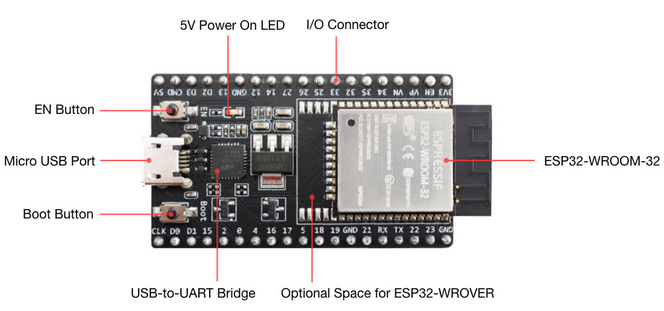
\includegraphics[scale=.5]{./Figures/devkit.png}
	\caption{ESP32-DevKitC V4 con el módulo ESP32-WROOM-32 integrado.}
	\label{fig:devkit}
\end{figure}


\subsection{Módulo sensor PH-4502C}
El sensor de pH analógico PH-4502C, figura \ref{fig:ph}, es un módulo electrónico diseñado para medir el grado de acidez de soluciones líquidas, típicamente el modelo E201-BNC \cite{PH:4502C}. Este sensor proporciona una salida de tensión analógica que es proporcional al nivel de pH detectado por el electrodo.

Características:

\begin{itemize}
	\item Módulo electrónico compatible con electrodos de pH con conector BNC.
	\item Rango de detección de pH de 0 a 14.
	\item Salida analógica que varía, entre 0 y 5 VDC, con el pH del liquido.
	\item Requiere una alimentación de voltaje de 5V DC.
	\item Corriente de operación entre 5 y 10 mA.
	\item Temperatura de operación del módulo generalmente entre -10 °C y 50 °C.
	\item Incorpora un potenciómetro para el ajuste del offset o calibración.
	\item El electrodo tiene un tiempo de estabilización de respuesta de aproximadamente 1 minuto.
\end{itemize}

\begin{figure}[h]
\centering
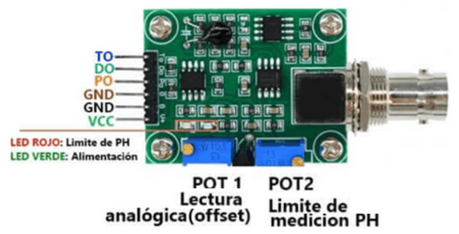
\includegraphics[scale=.5]{./Figures/ph.png}
	\caption{Distribución de pines del módulo PH-4502C.}
	\label{fig:ph}
\end{figure}

%https://uelectronics.com/producto/sensor-de-ph-liquido/?srsltid=AfmBOop9186NUUqLe2lmdM_tZTSfz79gsdcGSMFpg6aQvBxj-Fu9oF5t

\subsection{Módulo medidos de solidos disueltos totales}

El medidor de sólidos disueltos totales o TDS (del inglés \textit{Total Dissolved Solids}) Meter 1.0, figura \ref{fig:tds}, es un sensor o módulo electrónico diseñado para medir la cantidad total de sustancias orgánicas e inorgánicas disueltas en un líquido, expresada típicamente en partes por millón (ppm) o miligramos por litro (mg/l) \cite{TDS}. Este tipo de sensor se utiliza para evaluar la calidad del agua en diversas aplicaciones como hidroponía, acuicultura, tratamiento de aguas y monitoreo ambiental.

Características:

\begin{itemize}
	\item Requiere alimentación de 3.3 a 5.5 VDC.
	\item Salida analógica de 0 a 2.3 VDC (proporcional a TDS).
	\item Rango de medición típico de 0 a 1000 ppm.
	\item Incluye sonda impermeable con electrodos.
	\item Interfaz de 3 pines (VCC, GND, output).
	\item Conector para la sonda (2 pines).
	\item Compensación de temperatura.
\end{itemize}


\begin{figure}[h]
\centering
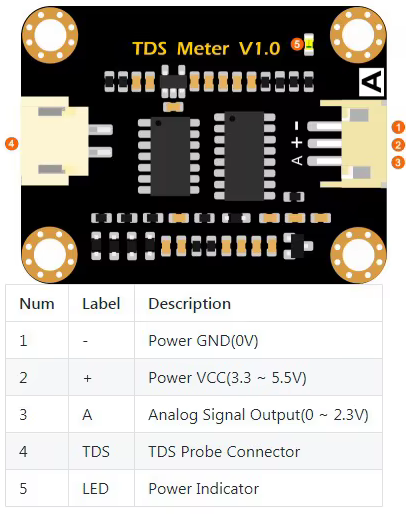
\includegraphics[scale=.5]{./Figures/tds.png}
	\caption{Ilustración del módulo sensor TDS meter v1.0.}
	\label{fig:tds}
\end{figure}

\subsection{Sensor de humedad capacitivo V2.0}

El sensor de humedad capacitivo V2.0, figura \ref{fig:moisture}, mide los niveles de humedad del medio mediante detección capacitiva en lugar de resistiva, como otros sensores disponibles. Fabricado con material resistente a la corrosión, ofrece una vida útil prolongada al insertarse en el sustrato alrededor de las plantas \cite{MOISTURE}.

\begin{itemize}
	\item Requiere alimentación de 3.3 a 5.5 VDC.
	\item Corriente de operación de 5 mA.
	\item Salida analógica.
	\item Incluye un regulador de tensión integrado compatible con MCUs de 3.3V y 5V.
\end{itemize}


\begin{figure}[h]
\centering
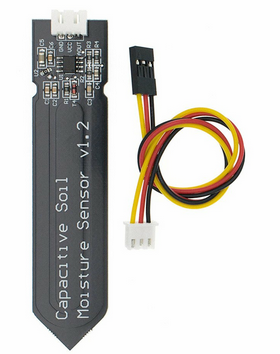
\includegraphics[scale=.5]{./Figures/moisture.png}
	\caption{Módulo sensor de humedad capacitivo.}
	\label{fig:moisture}
\end{figure}

\subsection{Sensor de temperatura digital DS18B20}

El DS18B20, figura \ref{fig:ds18b20}, es un sensor de temperatura digital que proporciona mediciones en grados celsius con una resolución configurable de 9 a 12 bits \cite{DS18B20}. Este sensor se comunica a través de un bus 1-Wire, lo que significa que solo requiere una línea de datos (además de tierra) para la comunicación con un micontrolador. Cada DS18B20 tiene un código de serie único de 64 bits grabado en fábrica, lo que permite que múltiples sensores funcionen en el mismo bus 1-Wire, lo que permite la creación de redes de sensores de temperatura distribuidos.

Características:

\begin{itemize}
	\item Requiere alimentación de 3.3 a 5.5 VDC.
	\item Rango de medición de temperatura: -55 °C a +125 °C (-67 °F a +257 °F).
	\item Precisión: ±0.5 °C en el rango de -10 °C a +85 °C.
	\item Resolución configurable: 9, 10, 11 o 12 bits (por defecto 12 bits).
	\item Interfaz de comunicación: 1-Wire (requiere un solo pin digital).
	\item Cada sensor tiene una dirección única de 64 bits.
	\item Puede alimentarse a través de la línea de datos (\textit{parasite power}) o con una fuente externa.
	\item Tiempo de conversión de temperatura: hasta 750 ms (para resolución de 12 bits).
	\item Disponible en encapsulado TO-92 y en versiones con sonda impermeable.
\end{itemize}


\begin{figure}[h]
\centering
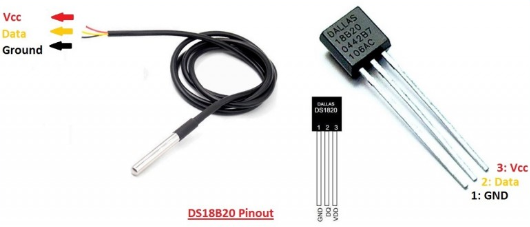
\includegraphics[scale=.5]{./Figures/ds18b20.png}
	\caption{Pinout del sensor DS18B20 y presentación del chip con su vaina protectora característica.}
	\label{fig:ds18b20}
\end{figure}

%https://tienda.ityt.com.ar/sensor-temp-hum-ic/1694-sensor-temperatura-ds18b20-18b20-1-wire-one-wire-itytarg.html

\subsection{Sensor de luz ambiental digital BH1750}

El circuito integrado BH1750, figura \ref{fig:BH1750}, es un sensor de luz ambiental digital con interfaz de bus I2C (\textit{Inter-Integrated Circuit}) \cite{BH1750}. Este sensor es capaz de detectar un amplio rango de intensidad luminosa con alta resolución, desde 1 hasta 65535 lux. El chip proporciona una salida digital directa, eliminando la necesidad de cálculos complejos.

\begin{itemize}
	\item Requiere alimentación de 3.3 a 5.5 VDC.
	\item Interfaz de comunicación I2C.
	\item Rango de medición de 1 a 65535 lux.
	\item Resolución: 16 bits.
\end{itemize}

\begin{figure}[h]
\centering
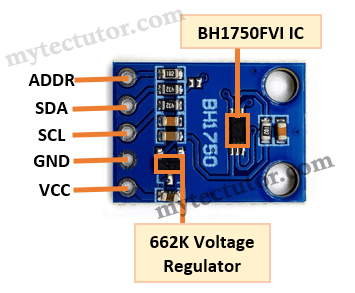
\includegraphics[scale=.5]{./Figures/BH1750.png}
	\caption{Pinout del módulo de adaptación del sensor BH1750.}
	\label{fig:BH1750}
\end{figure}

%https://mytectutor.com/bh1750-ambient-light-sensor-with-arduino/


\section{Componentes principales del software}
\label{sec:sw:components}
En esta sección se describen las herramientas de software de terceros utilizados en el trabajo.


\subsection{ESP-IDF}

ESP-IDF (\textit{Espressif IoT Development Framework}) es un conjunto de herramientas de desarrollo integral provisto por Espressif Systems. Este framework facilita la creación de firmware para su línea de SoCs ESP32 y ESP8266. Incluye un sistema operativo en tiempo real (FreeRTOS), bibliotecas con APIs para diversos periféricos y protocolos (Wi-Fi, bluetooth, TCP/IP), compilador (basado en GCC), depurador (GDB) y utilidades para la construcción, flasheo y monitoreo de proyectos. ESP-IDF permite a los desarrolladores escribir aplicaciones en C o C++, quienes aprovechan así la potencia y la conectividad de los chips de Espressif \cite{ESPIDF}.


\subsection{FreeRTOS}

FreeRTOS es un sistema operativo en tiempo real (RTOS) popular y de código abierto. Ofrece un núcleo pequeño y eficiente, apropiado para microcontroladores y sistemas con recursos limitados. Proporciona mecanismos de multitarea, como hilos (tareas), gestión de memoria, sincronización y comunicación entre tareas (semáforos, mutexes, colas). Facilita la organización y la gestión de la ejecución de múltiples funciones de manera concurrente y determinista, crucial para aplicaciones de tiempo real. Su portabilidad permite su uso en una amplia variedad de arquitecturas de procesadores \cite{FREERTOS}.

\subsection{Ceedling}

Ceedling es un framework de construcción y prueba para proyectos de software embebido en C. Automatiza tareas como la compilación, el enlazado y la ejecución de pruebas unitarias. Integra herramientas como Unity (para escribir pruebas), CMock (para crear objetos simulados) y Ruby (como lenguaje de automatización). Facilita la adopción de prácticas de desarrollo basadas en pruebas (TDD) y asegura la calidad del código mediante la verificación automatizada de unidades de software individuales. Proporciona una estructura organizada para la gestión de pruebas y la generación de informes \cite{CEEDLING}.

\subsection{React Native}
React Native es un framework de código abierto desarrollado por Meta. Permite la creación de aplicaciones móviles para plataformas iOS y Android desde una única base de código JavaScript. Utiliza los mismos bloques de construcción de la interfaz de usuario que las aplicaciones nativas. Esto resulta en aplicaciones con apariencia y rendimiento nativos. Una gran comunidad y un amplio ecosistema de bibliotecas lo respaldan \cite{reactnative}.

\section{Protocolos de comunicación empleados}

A continuación de detallan los protocolos de comunicación empleados en la realización del trabajo.

\subsection{HTTP}
HTTP (\textit{Hypertext Transfer Protocol}) es un protocolo de aplicación fundamental para la red de internet mundial. Define cómo los clientes (navegadores web) solicitan recursos (páginas web, imágenes, etc.) a los servidores y cómo estos responden. Utiliza un modelo de petición-respuesta. Las peticiones HTTP incluyen un método (GET, POST, PUT, DELETE, etc.) que indica la acción que el cliente desea realizar. Las respuestas HTTP contienen un código de estado que informa sobre el resultado de la petición. HTTP es un protocolo sin estado, lo que significa que cada petición es independiente de las anteriores \cite{HTTP}.

\subsection{I2C}
I2C (Inter-Integrated Circuit) es un protocolo de comunicación serial síncrono, multi-maestro/esclavo, de baja velocidad y corta distancia. Utiliza solo dos líneas bidireccionales: SDA (datos seriales) y SCL (reloj serial), ambas conectadas a través de resistencias pull-up. Permite que múltiples dispositivos (maestros y esclavos) se comuniquen entre sí en el mismo bus. Cada dispositivo es direccionable por un identificador único de 7 o 10 bits. Los maestros inician la comunicación y controlan el reloj, mientras que los esclavos responden a las peticiones de los maestros. Es ampliamente utilizado para conectar microcontroladores con periféricos de baja velocidad como sensores, EEPROMs y pantallas \cite{I2C}.

\subsection{1-Wire}
1-Wire es un protocolo de comunicación serial semidúplex diseñado por Dallas Semiconductor (ahora Analog Devices). Utiliza un único conductor para la comunicación de datos y, en algunos casos, para la alimentación. Un maestro controla la comunicación con uno o varios dispositivos esclavos en el mismo bus. Cada dispositivo es identificado por un código único de 64 bits grabado en fábrica. El protocolo es relativamente lento pero resulta económico para conectar sensores, memorias y otros dispositivos de baja velocidad, especialmente en aplicaciones donde el bajo número de pines es limitado. Permite la alimentación de los dispositivos esclavos a través de la línea de datos \cite{1WIRE}.










\section{xxxxxxxxxx}


Si en el texto se hace alusión a diferentes partes del trabajo referirse a ellas como capítulo, sección o subsección según corresponda. Por ejemplo: ``En el capítulo \ref{Chapter1} se explica tal cosa'', o ``En la sección \ref{sec:ejemplo} se presenta lo que sea'', o ``En la subsección \ref{subsec:ejemplo} se discute otra cosa''.

Cuando se quiere poner una lista tabulada, se hace así:

\begin{itemize}
	\item Este es el primer elemento de la lista.
	\item Este es el segundo elemento de la lista.
\end{itemize}

Notar el uso de las mayúsculas y el punto al final de cada elemento.

Si se desea poner una lista numerada el formato es este:

\begin{enumerate}
	\item Este es el primer elemento de la lista.
	\item Este es el segundo elemento de la lista.
\end{enumerate}

Notar el uso de las mayúsculas y el punto al final de cada elemento.

\subsection{Este es el título de una subsección}
\label{subsec:ejemplo}

Se recomienda no utilizar \textbf{texto en negritas} en ningún párrafo, ni tampoco texto \underline{subrayado}. En cambio sí se debe utilizar \textit{texto en itálicas} para palabras en un idioma extranjero, al menos la primera vez que aparecen en el texto. En el caso de palabras que estamos inventando se deben utilizar ``comillas'', así como también para citas textuales. Por ejemplo, un \textit{digital filter} es una especie de ``selector'' que permite separar ciertos componentes armónicos en particular.

La escritura debe ser impersonal. Por ejemplo, no utilizar ``el diseño del firmware lo hice de acuerdo con tal principio'', sino ``el firmware fue diseñado utilizando tal principio''. 

El trabajo es algo que al momento de escribir la memoria se supone que ya está concluido, entonces todo lo que se refiera a hacer el trabajo se narra en tiempo pasado, porque es algo que ya ocurrió. Por ejemplo, "se diseñó el firmware empleando la técnica de test driven development".

En cambio, la memoria es algo que está vivo cada vez que el lector la lee. Por eso transcurre siempre en tiempo presente, como por ejemplo:

``En el presente capítulo se da una visión global sobre las distintas pruebas realizadas y los resultados obtenidos. Se explica el modo en que fueron llevados a cabo los test unitarios y las pruebas del sistema''.

Se recomienda no utilizar una sección de glosario sino colocar la descripción de las abreviaturas como parte del mismo cuerpo del texto. Por ejemplo, RTOS (\textit{Real Time Operating System}, Sistema Operativo de Tiempo Real) o en caso de considerarlo apropiado mediante notas a pie de página.

Si se desea indicar alguna página web utilizar el siguiente formato de referencias bibliográficas, dónde las referencias se detallan en la sección de bibliografía de la memoria, utilizado el formato establecido por IEEE en \citep{IEEE:citation}. Por ejemplo, ``el presente trabajo se basa en la plataforma EDU-CIAA-NXP \citep{CIAA}, la cual...''.

\subsection{Figuras} 

Al insertar figuras en la memoria se deben considerar determinadas pautas. Para empezar, usar siempre tipografía claramente legible. Luego, tener claro que \textbf{es incorrecto} escribir por ejemplo esto: ``El diseño elegido es un cuadrado, como se ve en la siguiente figura:''

\begin{figure}[h]
\centering
\includegraphics[scale=.45]{./Figures/cuadradoAzul.png}
\end{figure}

La forma correcta de utilizar una figura es con referencias cruzadas, por ejemplo: ``Se eligió utilizar un cuadrado azul para el logo, como puede observarse en la figura \ref{fig:cuadradoAzul}''.

\begin{figure}[ht]
	\centering
	\includegraphics[scale=.45]{./Figures/cuadradoAzul.png}
	\caption{Ilustración del cuadrado azul que se eligió para el diseño del logo.}
	\label{fig:cuadradoAzul}
\end{figure}

El texto de las figuras debe estar siempre en español, excepto que se decida reproducir una figura original tomada de alguna referencia. En ese caso la referencia de la cual se tomó la figura debe ser indicada en el epígrafe de la figura e incluida como una nota al pie, como se ilustra en la figura \ref{fig:palabraIngles}.

\begin{figure}[htpb]
	\centering
	\includegraphics[scale=.3]{./Figures/word.jpeg}
	\caption{Imagen tomada de la página oficial del procesador\protect\footnotemark.}
	\label{fig:palabraIngles}
\end{figure}

\footnotetext{Imagen tomada de \url{https://goo.gl/images/i7C70w}}

La figura y el epígrafe deben conformar una unidad cuyo significado principal pueda ser comprendido por el lector sin necesidad de leer el cuerpo central de la memoria. Para eso es necesario que el epígrafe sea todo lo detallado que corresponda y si en la figura se utilizan abreviaturas entonces aclarar su significado en el epígrafe o en la misma figura.



\begin{figure}[ht]
	\centering
	\includegraphics[scale=.37]{./Figures/questionMark.png}
	\caption{¿Por qué de pronto aparece esta figura?}
	\label{fig:questionMark}
\end{figure}

Nunca colocar una figura en el documento antes de hacer la primera referencia a ella, como se ilustra con la figura \ref{fig:questionMark}, porque sino el lector no comprenderá por qué de pronto aparece la figura en el documento, lo que distraerá su atención.

Otra posibilidad es utilizar el entorno \textit{subfigure} para incluir más de una figura, como se puede ver en la figura \ref{fig:three graphs}. Notar que se pueden referenciar también las figuras internas individualmente de esta manera: \ref{fig:1de3}, \ref{fig:2de3} y \ref{fig:3de3}.
 
\begin{figure}[!htpb]
     \centering
     \begin{subfigure}[b]{0.3\textwidth}
         \centering
         \includegraphics[width=.65\textwidth]{./Figures/questionMark}
         \caption{Un caption.}
         \label{fig:1de3}
     \end{subfigure}
     \hfill
     \begin{subfigure}[b]{0.3\textwidth}
         \centering
         \includegraphics[width=.65\textwidth]{./Figures/questionMark}
         \caption{Otro.}
         \label{fig:2de3}
     \end{subfigure}
     \hfill
     \begin{subfigure}[b]{0.3\textwidth}
         \centering
         \includegraphics[width=.65\textwidth]{./Figures/questionMark}
         \caption{Y otro más.}
         \label{fig:3de3}
     \end{subfigure}
        \caption{Tres gráficos simples.}
        \label{fig:three graphs}
\end{figure}

El código para generar las imágenes se encuentra disponible para su reutilización en el archivo \file{Chapter2.tex}.

\subsection{Tablas}

Para las tablas utilizar el mismo formato que para las figuras, sólo que el epígrafe se debe colocar arriba de la tabla, como se ilustra en la tabla \ref{tab:peces}. Observar que sólo algunas filas van con líneas visibles y notar el uso de las negritas para los encabezados.  La referencia se logra utilizando el comando \verb|\ref{<label>}| donde label debe estar definida dentro del entorno de la tabla.

\begin{verbatim}
\begin{table}[h]
	\centering
	\caption[caption corto]{caption largo más descriptivo}
	\begin{tabular}{l c c}    
		\toprule
		\textbf{Especie}     & \textbf{Tamaño} & \textbf{Valor}\\
		\midrule
		Amphiprion Ocellaris & 10 cm           & \$ 6.000 \\		
		Hepatus Blue Tang    & 15 cm           & \$ 7.000 \\
		Zebrasoma Xanthurus  & 12 cm           & \$ 6.800 \\
		\bottomrule
		\hline
	\end{tabular}
	\label{tab:peces}
\end{table}
\end{verbatim}


\begin{table}[h]
	\centering
	\caption[caption corto]{caption largo más descriptivo.}
	\begin{tabular}{l c c}    
		\toprule
		\textbf{Especie} 	 & \textbf{Tamaño} 		& \textbf{Valor}  \\
		\midrule
		Amphiprion Ocellaris & 10 cm 				& \$ 6.000 \\		
		Hepatus Blue Tang	 & 15 cm				& \$ 7.000 \\
		Zebrasoma Xanthurus	 & 12 cm				& \$ 6.800 \\
		\bottomrule
		\hline
	\end{tabular}
	\label{tab:peces}
\end{table}

En cada capítulo se debe reiniciar el número de conteo de las figuras y las tablas, por ejemplo, figura 2.1 o tabla 2.1, pero no se debe reiniciar el conteo en cada sección. Por suerte la plantilla se encarga de esto por nosotros.

\subsection{Ecuaciones}
\label{sec:Ecuaciones}

Al insertar ecuaciones en la memoria dentro de un entorno \textit{equation}, éstas se numeran en forma automática  y se pueden referir al igual que como se hace con las figuras y tablas, por ejemplo ver la ecuación \ref{eq:metric}.

\begin{equation}
	\label{eq:metric}
	ds^2 = c^2 dt^2 \left( \frac{d\sigma^2}{1-k\sigma^2} + \sigma^2\left[ d\theta^2 + \sin^2\theta d\phi^2 \right] \right)
\end{equation}
                                                        
Es importante tener presente que si bien las ecuaciones pueden ser referidas por su número, también es correcto utilizar los dos puntos, como por ejemplo ``la expresión matemática que describe este comportamiento es la siguiente:''

\begin{equation}
	\label{eq:schrodinger}
	\frac{\hbar^2}{2m}\nabla^2\Psi + V(\mathbf{r})\Psi = -i\hbar \frac{\partial\Psi}{\partial t}
\end{equation}

Para generar la ecuación \ref{eq:metric} se utilizó el siguiente código:

\begin{verbatim}
\begin{equation}
	\label{eq:metric}
	ds^2 = c^2 dt^2 \left( \frac{d\sigma^2}{1-k\sigma^2} + 
	\sigma^2\left[ d\theta^2 + 
	\sin^2\theta d\phi^2 \right] \right)
\end{equation}
\end{verbatim}

Y para la ecuación \ref{eq:schrodinger}:

\begin{verbatim}
\begin{equation}
	\label{eq:schrodinger}
	\frac{\hbar^2}{2m}\nabla^2\Psi + V(\mathbf{r})\Psi = 
	-i\hbar \frac{\partial\Psi}{\partial t}
\end{equation}

\end{verbatim}